\subsection{Esercizio 6}
\lstinputlisting[language=Matlab]{capitolo2/es6.m}
Eseguendo lo script si ottengono i seguenti risultati:\\\\
\begin{itemize}
        \item Valore approssimato:\\
        \begin{tabular}{|l|l|l|l|l|}
                \hline
                Metodo & tolleranza$=10^{-3}$  & tolleranza$=10^{-6}$ & tolleranza$=10^{-9}$ & tolleranza$=10^{-12}$ \\
                \hline
                bisezione & 7.39257812500000e-01 &  7.39085197448730e-01  & 7.39085133187473e-01 &  7.39085133215667e-01\\
                newton   &  7.39085133385284e-01 &  7.39085133215161e-01  & 7.39085133215161e-01 & 7.39085133215161e-01 \\
                corde    &  7.39567202212256e-01  & 7.39084549575213e-01 & 7.39085132739254e-01 & 7.39085133215737e-01 \\
                secanti  &  7.39085133215001e-01  & 7.39085133215161e-01  &  7.39085133215161e-01  &  7.39085133215161e-01 \\
                \hline
                
        \end{tabular}
        \item 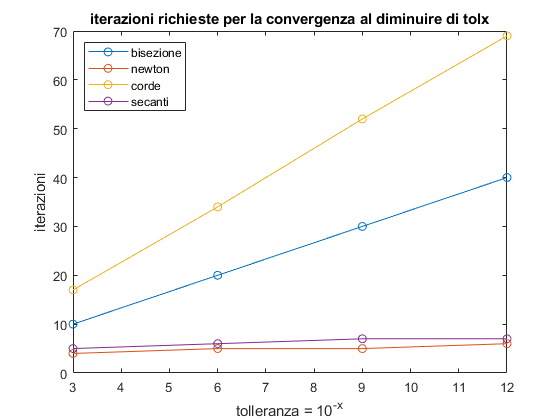
\includegraphics[scale=1]{capitolo2/iter.png}
\end{itemize}

